\documentclass[a4paper]{scrartcl}
\usepackage[utf8]{inputenc}
\usepackage{amsmath,amssymb,amsthm}
\usepackage{enumitem,setspace}
\usepackage[usenames,dvipsnames,table]{xcolor}
\usepackage{graphicx}
\DeclareGraphicsExtensions{.pdf,.png,.eps,.jpg}
\usepackage{algorithm2e}

% --- math operators ---
\usepackage{mathtools}
\DeclarePairedDelimiter\set{\{}{\}} % use $\set{1, 2, 3}$
\DeclarePairedDelimiter\abs{\lvert}{\rvert}
\DeclarePairedDelimiter\norm{\lVert}{\rVert}
\DeclarePairedDelimiter\ceils{\lceil}{\rceil}
\DeclarePairedDelimiter\floor{\lfloor}{\rfloor}
\def\then{\ensuremath{\Rightarrow}} % =>
\def\iff{\ensuremath{\Leftrightarrow}} % if and only if <=>
\def\to{\ensuremath{\rightarrow}} % ->
\def\ot{\ensuremath{\leftarrow}} % ->
\def\Oh{\ensuremath{\mathcal{O}}} % big O like $\Oh(n)$
% ---
\DeclareMathOperator{\preorder}{preorder}
\DeclareMathOperator{\postorder}{postorder}
\DeclareMathOperator{\depth}{depth}

% --- FILL OUT THESE 3 FIELDS ---
\def\sheetNumber{1}
\def\names{Matthias Janßen} 
\def\sumPoints{20} 

% --- ### BEGIN DOCUMENT ### ---
\begin{document} 

\begin{doublespace} % header
\noindent \textbf{\LARGE{Übungsblatt \sheetNumber}}
\hfill  {\large Punkte: $\boxed{\qquad  /\; \sumPoints}$}\\
{\Large \textbf{Fortgeschrittene Algorithmen (Wintersemester 2022/23)}\\
Bearbeitet von: \textbf{\names}\\
\today}
\end{doublespace}


\section*{Aufgabe 1}
MaxProben(int[][] A, int m, int n)
\begin{verbatim}
    //Merken aus welcher Richtung der Rover kommt
    char previous[m][n]
    //Matrix durchlaufen
    for i = 1 to m do
        for j = 1 to n do
            //Startfeld braucht keine Aktion
            if(i == 1 & j == 1) then skip
            //Am linken Rand kann der vorherige Punkt nur oben ('O') liegen
            else if(i == 1) then
                //Die Summe des vorherigen und aktuellen Knoten wird gespeichert, 
                //so wird der gesamte Wert des Weges gezählt
                A[i][j] = A[i][j] + A[i][j-1]
                previous[i][j] = 'O'
            //Am oberen Rand kann der vorherige Punkt nur links ('L') liegen
            else if(j == 1) then
                A[i][j] = A[i][j] + A[i-1][j]
                previous[i] = 'L'
            else
                //Je nachdem ob die Summe des Weges von "oben" oder "links" und des aktuellen Knoten größer ist
                //wird der Vorgänger und Wert gespeichert
                max = A[i][j] + A[i-1][j]
                if A[i][j] + A[i][j-1] > max then
                    max = A[i][j] + A[i][j-1]
                    previous[i][j] = 'L'
                else
                    previous[i][j] = 'O'
                A[i][j] = max
    //Pfad rekonstruieren indem von hinten nach vorne gegangen wird
    path = []
    while not (m == 1 & n == 1) do
        if previous[m][n] == 'L' then
            m = m - 1
            //'o' für Osten
            path.add('s')
        else
            n = n - 1
            //'s' für Süden
            path.add('o')
    return path.reverse, A

\end{verbatim}

Der Algorithmus läuft in $\Oh(m \cdot n)$ Zeit, da jedes Feld der Matrix genau einmal besucht wird.\bigskip\newline
\section*{Aufgabe 2}

a)

\begin{figure}[htb]
\centering

\includegraphics[width=0.6\linewidth]{greedy_kurz.png} % use option [width=\linewidth] to change size to linewidth (or 0.6\linewidth for example)
\caption{Auswahl des Algorithmus}
\label{fig:greedy_a}
\end{figure}

Der Greedy Algorithmus aus Aufgabe a wählt die erste Aufgabe da sie die kürzeste ist. Dadurch kann nur eine Aufgabe
gewählt werden, auch wenn es möglich wäre 2 Aufträge zu erledigen.
\bigskip\newline 
b)

\begin{figure}[htb]
\centering
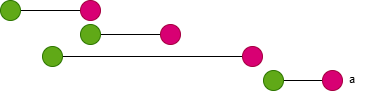
\includegraphics[width=0.6\linewidth]{Greedy_überlappen.png} % use option [width=\linewidth] to change size to linewidth (or 0.6\linewidth for example)
\caption{Auswahl des Algorithmus}
\label{fig:greedy_b}
\end{figure}

Der Algorithmus wählt nur den letzten Auftrag a da dieser mit keinem anderem überlappt.
\bigskip\newline
c) 

\begin{figure}[htb]
\centering
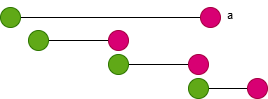
\includegraphics[width=0.6\linewidth]{Greedy_frühester.png} % use option [width=\linewidth] to change size to linewidth (or 0.6\linewidth for example)
\caption{Auswahl des Algorithmus}
\label{fig:greedy_c}
\end{figure}

Der Algorithmus wählt Auftrag a da dieser den frühesten Startzeitpunkt hat. Dadurch kann nur ein Auftrag ausgewählt werden,
obwohl 3 möglich wären. \pagebreak
\section*{Aufgabe 3}
a)
\begin{verbatim}
GreedyTimer(int[] t, int z)
    L = { }
    while z > 0
        for m = 0 to t.length do
            if t[m] > z
                L.add[t[m-1]]
                z = z - t[m-1]
                m = 0
            if m == t.length
                L.add[t[m]]
                z = z - t[m]
                m = 0
    return L
    
\end{verbatim}
Der Algorithmus wählt immer die größte Taste aus die in die verbleibende Zeit passt. Da alle Tasten außer 1 den Teiler 5 Teilen 
wird so immer der optimale Weg gefunden.\bigskip

b)
Ein Pizzaofen mit den Tasten 1, 5 \& 6. Für eine Eingabe von 10 Sekunden würde ein Greedy Algorithmus der immer die größtmögliche
Taste wählt die Tastenkombination 6, 1, 1, 1, 1  auswählen asntatt 5, 5.

%\section*{Aufgabe 4}


% -- code for figures
% \begin{figure}[htb]
% \centering
% \includegraphics{filename} % use option [width=\linewidth] to change size to linewidth (or 0.6\linewidth for example)
% \label{fig:name}
% \end{figure}


\end{document}
% --- ### END DOCUMENT ### ---